\section{Project Management}
\label{sec:project_management}
\lhead{\thesection \space Project Management}

TODO Patrick


%%%%%%%%%%%%%%%%%%%%%%%%%%%%%%%%%%%%%%%%%%%%%%%%%%
%% INTEGRATION MANAGEMENT
%%%%%%%%%%%%%%%%%%%%%%%%%%%%%%%%%%%%%%%%%%%%%%%%%%

\subsection{Integration Management}
\label{ssec:integration_management}

TODO Patrick


%%%%%%%%%%%%%%%%%%%%%%%%%%%%%%%%%%%%%%%%%%%%%%%%%%
%% SCOPE MANAGEMENT
%%%%%%%%%%%%%%%%%%%%%%%%%%%%%%%%%%%%%%%%%%%%%%%%%%

\subsection{Scope Management}
\label{ssec:scope_management}

Scope management is what you do to make sure that your project includes all the work relevant to achieving the project’s objectives and not anything else. It’s about controlling what’s included in the project and what is not.

\subsubsection{Plan Scope Management}
\label{sssec:plan_scope_management}

This project is for designing, programming, and testing a new software product which will be a new module of the connected.football app to add a feature to vote on given exercises. This includes design of the software, all programming and coding, and testing/validation of the software.
\newline
For this project, scope management will be the sole responsibility of all group members. The scope for this project is defined by the Scope Statement, Work Breakdown Structure and the Software Requirement Specification. Proposed scope changes may be initiated by the product owner as well as every member of the team.

\begin{table}[H]
    \centering
    \begin{tabular}{|c|c|l|}
        \hline
        \cellcolor{gray}Name & 
        \cellcolor{gray}Role &
        \cellcolor{gray}Responsibilities \\\hline
        Guido Budziak & Product owner &- Approve or deny scope changes.\\&&- Evaluate need for scope change requests.\\&&- Accept project deliverables\\\hline
        Lucas Gehlen&Team member&- Measure and verify project scope.\\
        Marco Kull&&- Update project documents upon scope changes.\\
        Patrick Richter&&- Measure and verify project scope.\\
        Sebastian Wilczek&&- Participate in defining change resolutions.\\
        &&- Evaluate the need for scope changes.\\\hline
    \end{tabular}
    \caption{Scope Roles \& Responsibilities}
    \label{tab:scope_roles}
\end{table}

\subsubsection{Collect Requirements}
\label{sssec:collect_requirements}

The requirements for this project are delivered by the product owner. During the weekly meetings with the product owner the team will discuss the design fragments with him to ensure the requirements are met. All requirements will be documented in a software requirement specification document.

\subsubsection{Define Scope}
\label{sssec:define_scope}

This project includes the design, programming, and testing of a new module of the connected.football app to add a feature to vote on given exercises. The deliverables for this project is a completed module with the flexibility to modify and expand as necessary in the future. This project will be accepted once the new module has been successfully tested. Assumptions for this project are that support will be provided by the project owner.

\subsubsection{Create WBS}
\label{sssec:create_wbs}

The project is broken down into three phases: Vote4Fun; Promotion Code; and Vote4Fun Group Extension. Each of these phases is then subdivided further down.

\begin{figure}[H]
	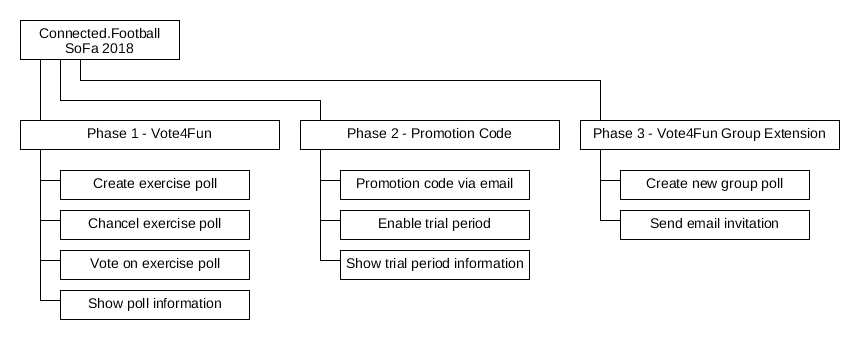
\includegraphics[width=\textwidth]{images/wbs.png}
	\caption{Work Breakdown Structure}
    \label{fig:wbs}
\end{figure}

\subsubsection{Validate Scope}
\label{sssec:validate_scope}
    
As this project progresses the team will verify interim project deliverables against the original scope. To ensure that project work remains within the scope of the project those interim deliverables will be discussed in weekly meetings with the product owner.

\subsubsection{Control Scope}
\label{sssec:control_scope}

The project team will work together to control of the scope of the project. The project manager will oversee the project team and the progression of the project to ensure that this scope control process if followed.
\newline
If a change to the project scope is needed, all team members and the product owner must approve of the scope change.

%%%%%%%%%%%%%%%%%%%%%%%%%%%%%%%%%%%%%%%%%%%%%%%%%%
%% TIME MANAGEMENT
%%%%%%%%%%%%%%%%%%%%%%%%%%%%%%%%%%%%%%%%%%%%%%%%%%

\subsection{Time Management}
\label{ssec:time_management}

TODO Patrick


%%%%%%%%%%%%%%%%%%%%%%%%%%%%%%%%%%%%%%%%%%%%%%%%%%
%% COST MANAGEMENT
%%%%%%%%%%%%%%%%%%%%%%%%%%%%%%%%%%%%%%%%%%%%%%%%%%

\subsection{Cost Management}
\label{ssec:cost_management}

This subsection deals with the cost management of the project in question. It is being detailed how cost were managed in the project and how costs and expenses were monitored over the course of the project.
\newline
Costs did not play a vital role in the project. Given that the project is part of a University module, the project team is working without compensation and all resources, such as they are mentioned in \textit{Subsection \ref{ssec:procurement_management}}, are being provided by the client.
\newline
Cost management was considered during the project planning due to the small likelihood that the project requires further resources. In this case, the responsibility for providing these resources were that of the client. However, the project team would have been responsible for defining why the new resource is necessary for development and on what scale the resource needs to be provided. However, such a case never occurred during the course of the project is only mentioned for the purpose of completeness.


%%%%%%%%%%%%%%%%%%%%%%%%%%%%%%%%%%%%%%%%%%%%%%%%%%
%% STAKEHOLDER MANAGEMENT
%%%%%%%%%%%%%%%%%%%%%%%%%%%%%%%%%%%%%%%%%%%%%%%%%%

\subsection{Stakeholder Management}
\label{ssec:stakeholder_management}

TODO Lucas


%%%%%%%%%%%%%%%%%%%%%%%%%%%%%%%%%%%%%%%%%%%%%%%%%%
%% HUMAN RESOURCE MANAGEMENT MANAGEMENT
%%%%%%%%%%%%%%%%%%%%%%%%%%%%%%%%%%%%%%%%%%%%%%%%%%

\subsection{Human Resource Management}
\label{ssec:human_resource_management}

TODO Patrick


%%%%%%%%%%%%%%%%%%%%%%%%%%%%%%%%%%%%%%%%%%%%%%%%%%
%% COMMUNICATION MANAGEMENT
%%%%%%%%%%%%%%%%%%%%%%%%%%%%%%%%%%%%%%%%%%%%%%%%%%

\subsection{Communication Management}
\label{ssec:communication_management}

TODO Lucas


%%%%%%%%%%%%%%%%%%%%%%%%%%%%%%%%%%%%%%%%%%%%%%%%%%
%% RISK MANAGEMENT
%%%%%%%%%%%%%%%%%%%%%%%%%%%%%%%%%%%%%%%%%%%%%%%%%%

\subsection{Risk Management}
\label{ssec:risk_management}

TODO Patrick


%%%%%%%%%%%%%%%%%%%%%%%%%%%%%%%%%%%%%%%%%%%%%%%%%%
%% PROCUREMENT MANAGEMENT
%%%%%%%%%%%%%%%%%%%%%%%%%%%%%%%%%%%%%%%%%%%%%%%%%%

\subsection{Procurement Management}
\label{ssec:procurement_management}

Part of the Project Management process is to manage the processes necessary to acquire services and products that ensure the ability to work on the project. This includes both management services as well as external software products used in development.
\newline
The project encompassed the following products and services. It is detailed how they were used in the project and who was responsible for providing them.

\subsubsection{Atlassian \textit{Jira}}
\label{sssec:jira}

\begin{figure}[H]
    \begin{center}
        
\includegraphics[width=0.3\textwidth]{images/logos/jira-logo.png}
        \caption{Atlassian \textit{Jira} Logo}
        \label{fig:jira_logo}
    \end{center}
\end{figure}

To manage the agile process of the project, \textit{Jira} by Atlassian was made use of. The platform allowed the project team members to keep track of the backlog of tasks and user stories and to manage them in Scrum sprints.
\newline
\textit{Jira} was provided by the client \textit{Connected.Football}. The client was responsible for granting the other team members and stakeholders access to the tool and to ensure that certain team members have the necessary permissions to interact with the provided tool set. The developing team members were responsible for keeping the content of the created \textit{Jira} boards correct and up-to-date.

\subsubsection{\textit{GitHub}}
\label{sssec:github}

\begin{figure}[H]
    \begin{center}
        
\includegraphics[width=0.2\textwidth]{images/logos/github-logo.png}
        \caption{\textit{GitHub} Logo}
        \label{fig:github_logo}
    \end{center}
\end{figure}

The developed \textit{React Native} product was being versioned using \textit{Git}, which uses \textit{GitHub} as a platform. The client was again responsible for providing the team members access to the versioning system and to ensure that the provided sources are in a state that enables development by the project team.
\newline
The project team was responsible for committing changes they make to the product to the \textit{GitHub} repository, including accurate descriptions of what has been changed since the last commit. It was also the responsibility of the team to resolve commit errors and conflicts, as well as to minimise the likelihood of such occurrences.

\subsubsection{\textit{Subversion}}
\label{sssec:subversion}

Another versioning system used over the course of the project was \textit{Subversion}. This system was used to commit and share University-related artefacts and documents, such as this project report.
\newline
Fontys Hogeschool Techniek en Logistiek Venlo was responsible for the availability and integrity of the repositories in question. Again, it was the responsibility of the team members to ensure a working state of the repositories and to commit changes with accurate descriptions.

\subsubsection{\textit{Firebase}}
\label{sssec:firebase}

\begin{figure}[H]
    \begin{center}
        
\includegraphics[width=0.2\textwidth]{images/logos/firebase-logo.png}
        \caption{\textit{Firebase} Logo}
        \label{fig:firebase_logo}
    \end{center}
\end{figure}

Some backend functionality of the product was relying on Google's \textit{Firebase}. It was for example used to send push notifications to mobile user devices.
\newline
It was the responsibility of the client to ensure that the project team has the necessary rights to interact with the already set up \textit{Firebase} backend. On the other hand, the team was responsible for interacting with the backend in a proper way, ensuring the integrity of the provided data and infrastructure. The project team did not have any access to the backend in the sense of interacting with the interface provided by Google, but by using it by referencing and using it in the source code of the application.

\subsubsection{Integrated development environments}
\label{sssec:ides}

\begin{figure}[H]
    \begin{center}
        
\includegraphics[width=0.2\textwidth]{images/logos/visual-studio-code-logo.png}
        \caption{\textit{Visual Studio Code} Logo}
        \label{fig:visual-studio-code_logo}
    \end{center}
\end{figure}

The project team used some integrated development environments (IDEs) to develop the product, most notably \textit{Visual Studio Code}. The IDE was used to inspect and change the source code of the product.
\newline
The developer was responsible for the functionality of the IDE. The team was able to use the IDEs as they are all provided through open source. It was their responsibility to use the IDE as intended and to figure out how to resolve errors in the event that they occur. No such errors occurred during the course of the project.

\subsubsection{\textit{Node.js} Modules}
\label{sssec:nodejs_modules}

\begin{figure}[H]
    \begin{center}
        
\includegraphics[width=0.3\textwidth]{images/logos/node-js-logo.png}
        \caption{\textit{Node.js} Logo}
        \label{fig:node-js-logo}
    \end{center}
\end{figure}

The product used various \textit{Node.js} modules to offer functionality in the product. These modules were available from various repositories.
\newline
The developers of the \textit{Node.js} modules were responsible for the development of the \textit{Node.js} modules themselves and for the documentation that comes with them. Since the modules were published as open source, the project team is responsible for handling errors that occurred during the development involving their usage. They were furthermore responsible for implementing the usage of the modules in the product as the developer intended and documented.
\newline
Some of the \textit{Node.js} modules were developed by the client. Their integrity was therefore their responsibility.

\subsubsection{\textit{Slack}}
\label{sssec:slack}

\begin{figure}[H]
    \begin{center}
        
\includegraphics[width=0.2\textwidth]{images/logos/slack-logo.png}
        \caption{\textit{Slack} Logo}
        \label{fig:slack-logo}
    \end{center}
\end{figure}

The development team used \textit{Slack} to communicate outside of personal meetings, both in communication with each other as well as with the client. It was also used to share information, such as documents and source code snippets, in a non-persistent way. Configuration files that were not supposed to be uploaded to \textit{GitHub} were also shared using \textit{Slack}.
\newline
The availability of the application was ensured by the developer. It was the responsibility of the client to enable that the development team is able to join and use the \textit{Slack} platform. The project team had the responsibility to not share any sensitive information, such as credentials, over this platform.